%% LyX 2.1.3 created this file.  For more info, see http://www.lyx.org/.
%% Do not edit unless you really know what you are doing.
\documentclass[english]{article}
\usepackage[latin9]{inputenc}
\usepackage[a4paper]{geometry}
\geometry{verbose,tmargin=1in,bmargin=1in,lmargin=0.5in,rmargin=0.5in}
\usepackage{fancyhdr}
\pagestyle{fancy}
\setlength{\parskip}{\smallskipamount}
\setlength{\parindent}{0pt}
\usepackage{babel}
\usepackage{units}
\usepackage{amsmath}
\usepackage{amssymb}
\usepackage[unicode=true,
 bookmarks=true,bookmarksnumbered=false,bookmarksopen=false,
 breaklinks=false,pdfborder={0 0 0},backref=false,colorlinks=false]
 {hyperref}
\hypersetup{pdftitle={Trigonometry Cram Sheet},
 pdfauthor={All Too Technical}}

\makeatletter

%%%%%%%%%%%%%%%%%%%%%%%%%%%%%% LyX specific LaTeX commands.
%% Because html converters don't know tabularnewline
\providecommand{\tabularnewline}{\\}

%%%%%%%%%%%%%%%%%%%%%%%%%%%%%% Textclass specific LaTeX commands.
\newenvironment{lyxlist}[1]
{\begin{list}{}
{\settowidth{\labelwidth}{#1}
 \setlength{\leftmargin}{\labelwidth}
 \addtolength{\leftmargin}{\labelsep}
 \renewcommand{\makelabel}[1]{##1\hfil}}}
{\end{list}}

%%%%%%%%%%%%%%%%%%%%%%%%%%%%%% User specified LaTeX commands.
\usepackage{pgf,tikz}
\usepackage{mathrsfs}
\usetikzlibrary{arrows}
\usepackage{multicol}
\usepackage{array}
\usepackage{pgfplots}

\makeatother

\begin{document}

\lhead{\textsf{\textbf{Trigonometry Cram Sheet}}}


\rhead{\textsf{\href{http://www.alltootechnical.tk}{alltootechnical.tk}}}


\title{\textsf{\textbf{Trigonometry Cram Sheet}}}


\date{\textsf{October 27, 2015}}

\maketitle
\begin{multicols*}{2}

\tableofcontents{}

\end{multicols*}\newpage{}

\begin{multicols}{2}


\section{Definition}

Triangle $ABC$ has a right angle at $C$ and sides of length $a$,
$b$, $c$. The trigonometric functions of angle $A$ are defined
as follows:
\begin{enumerate}
\item ${\displaystyle \sin A=\frac{a}{c}=\frac{\mathrm{opposite}}{\mathrm{hypotenuse}}}$
\item ${\displaystyle \cos A=\frac{b}{c}=\frac{\mathrm{adjacent}}{\mathrm{hypotenuse}}}$
\item ${\displaystyle \tan A=\frac{a}{b}=\frac{\mathrm{opposite}}{\mathrm{adjacent}}}$
\item ${\displaystyle \csc A=\frac{b}{a}=\frac{\mathrm{hypotenuse}}{\mathrm{opposite}}}$
\item ${\displaystyle \sec A=\frac{c}{a}=\frac{\mathrm{hypotenuse}}{\mathrm{adjacent}}}$
\item ${\displaystyle \cot A=\frac{b}{a}=\frac{\mathrm{adjacent}}{\mathrm{opposite}}}$
\end{enumerate}

\subsection{Extensions to Angles $>90^{\circ}$}

A point $P$ in the Cartesian plane has coordinates $\left(x,y\right)$,
where $x$ is considered as positive along $OX$ and negative along
$OX'$, while $y$ is considered as positive along $OY'$ and negative
along $OY$. The distance from origin $O$ to point $P$ is positive
and denoted by $r=\sqrt{x^{2}+y^{2}}$. The angle $A$ described \emph{counterclockwise}
from $OX$ is considered \emph{positive}. If it is described \emph{clockwise}
from $OX$ it is considered \emph{negative}.

For an angle $A$ in any quadrant, the trigonometric functions of
$A$ are defined as follows:
\begin{enumerate}
\item ${\displaystyle \sin A=\frac{y}{r}}$
\item ${\displaystyle \cos A=\frac{x}{r}}$
\item ${\displaystyle \tan A=\frac{y}{x}}$
\item ${\displaystyle \csc A=\frac{r}{y}}$
\item ${\displaystyle \sec A=\frac{r}{x}}$
\item ${\displaystyle \cot A=\frac{x}{y}}$
\end{enumerate}

\subsection{The Unit Circle}

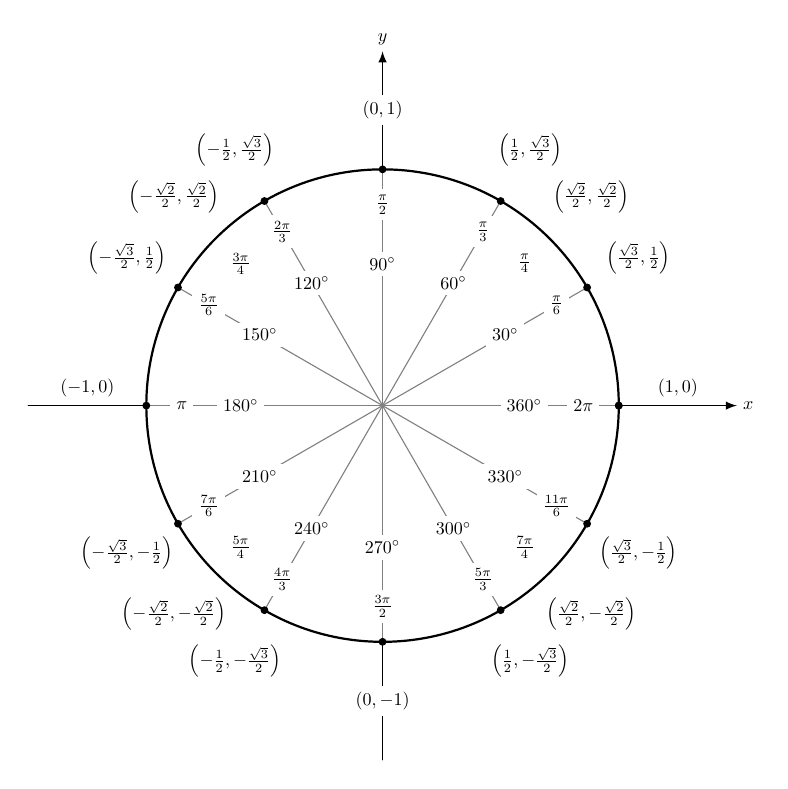
\begin{tikzpicture}[scale=3,cap=round,>=latex,every node/.style={scale=0.65}]
        % draw the coordinates
        \draw[->] (-1.5cm,0cm) -- (1.5cm,0cm) node[right,fill=white] {$x$};
        \draw[->] (0cm,-1.5cm) -- (0cm,1.5cm) node[above,fill=white] {$y$};

        % draw the unit circle
        \draw[thick] (0cm,0cm) circle(1cm);

        \foreach \x in {0,30,...,360} {
                % lines from center to point
                \draw[gray] (0cm,0cm) -- (\x:1cm);
                % dots at each point
                \filldraw[black] (\x:1cm) circle(0.4pt);
                % draw each angle in degrees
                \draw (\x:0.6cm) node[fill=white] {$\x^\circ$};
        }

        % draw each angle in radians
        \foreach \x/\xtext in {
            30/\frac{\pi}{6},
            45/\frac{\pi}{4},
            60/\frac{\pi}{3},
            90/\frac{\pi}{2},
            120/\frac{2\pi}{3},
            135/\frac{3\pi}{4},
            150/\frac{5\pi}{6},
            180/\pi,
            210/\frac{7\pi}{6},
            225/\frac{5\pi}{4},
            240/\frac{4\pi}{3},
            270/\frac{3\pi}{2},
            300/\frac{5\pi}{3},
            315/\frac{7\pi}{4},
            330/\frac{11\pi}{6},
            360/2\pi}
                \draw (\x:0.85cm) node[fill=white] {$\xtext$};

        \foreach \x/\xtext/\y in {
            % the coordinates for the first quadrant
            30/\frac{\sqrt{3}}{2}/\frac{1}{2},
            45/\frac{\sqrt{2}}{2}/\frac{\sqrt{2}}{2},
            60/\frac{1}{2}/\frac{\sqrt{3}}{2},
            % the coordinates for the second quadrant
            150/-\frac{\sqrt{3}}{2}/\frac{1}{2},
            135/-\frac{\sqrt{2}}{2}/\frac{\sqrt{2}}{2},
            120/-\frac{1}{2}/\frac{\sqrt{3}}{2},
            % the coordinates for the third quadrant
            210/-\frac{\sqrt{3}}{2}/-\frac{1}{2},
            225/-\frac{\sqrt{2}}{2}/-\frac{\sqrt{2}}{2},
            240/-\frac{1}{2}/-\frac{\sqrt{3}}{2},
            % the coordinates for the fourth quadrant
            330/\frac{\sqrt{3}}{2}/-\frac{1}{2},
            315/\frac{\sqrt{2}}{2}/-\frac{\sqrt{2}}{2},
            300/\frac{1}{2}/-\frac{\sqrt{3}}{2}}
                \draw (\x:1.25cm) node[fill=white] {$\left(\xtext,\y\right)$};

        % draw the horizontal and vertical coordinates
        % the placement is better this way
        \draw (-1.25cm,0cm) node[above=1pt] {$(-1,0)$}
              (1.25cm,0cm)  node[above=1pt] {$(1,0)$}
              (0cm,-1.25cm) node[fill=white] {$(0,-1)$}
              (0cm,1.25cm)  node[fill=white] {$(0,1)$};
    \end{tikzpicture}


\subsection{Degrees and Radians}

A \emph{radian} is that angle $\theta$ subtended at center $O$ of
a circle by an arc $MN$ equal to the radius $r$. Since $\unit[2\pi]{radians}=360\textdegree$
we have:
\begin{lyxlist}{00.00.0000}
\item [{$\unit[1]{radian}=180\textdegree/\pi=57.29577951308232\dots\textdegree$}]~
\item [{$1\textdegree=\unit[\pi/180]{radians}=\unit[0.017453292519943\dots]{radians}$}]~
\end{lyxlist}

\subsection{Signs and Variations}

\begin{tabular}{|c|c|c|c|}
\hline 
Quadrant & $\sin A$ & $\cos A$ & $\tan A$\tabularnewline
\hline 
\hline 
I & $\begin{array}{c}
+\\
\left(0,1\right)
\end{array}$ & $\begin{array}{c}
+\\
\left(1,0\right)
\end{array}$ & $\begin{array}{c}
+\\
\left(0,\infty\right)
\end{array}$\tabularnewline
\hline 
II & $\begin{array}{c}
+\\
\left(1,0\right)
\end{array}$ & $\begin{array}{c}
-\\
\left(0,-1\right)
\end{array}$ & $\begin{array}{c}
-\\
\left(-\infty,0\right)
\end{array}$\tabularnewline
\hline 
III & $\begin{array}{c}
-\\
\left(0,-1\right)
\end{array}$ & $\begin{array}{c}
-\\
\left(-1,0\right)
\end{array}$ & $\begin{array}{c}
+\\
\left(0,\infty\right)
\end{array}$\tabularnewline
\hline 
IV & $\begin{array}{c}
-\\
\left(-1,0\right)
\end{array}$ & $\begin{array}{c}
+\\
\left(0,1\right)
\end{array}$ & $\begin{array}{c}
-\\
\left(-\infty,0\right)
\end{array}$\tabularnewline
\hline 
\end{tabular}

\begin{tabular}{|c|c|c|c|}
\hline 
Quadrant & $\cot A$ & $\sec A$ & $\csc A$\tabularnewline
\hline 
\hline 
I & $\begin{array}{c}
+\\
\left(\infty,0\right)
\end{array}$ & $\begin{array}{c}
+\\
\left(1,\infty\right)
\end{array}$ & $\begin{array}{c}
+\\
\left(\infty,1\right)
\end{array}$\tabularnewline
\hline 
II & $\begin{array}{c}
-\\
\left(0,-\infty\right)
\end{array}$ & $\begin{array}{c}
-\\
\left(\infty,-1\right)
\end{array}$ & $\begin{array}{c}
+\\
\left(1,\infty\right)
\end{array}$\tabularnewline
\hline 
III & $\begin{array}{c}
+\\
\left(\infty,0\right)
\end{array}$ & $\begin{array}{c}
-\\
\left(-1,\infty\right)
\end{array}$ & $\begin{array}{c}
-\\
\left(\infty,-1\right)
\end{array}$\tabularnewline
\hline 
IV & $\begin{array}{c}
-\\
\left(0,-\infty\right)
\end{array}$ & $\begin{array}{c}
+\\
\left(\infty,1\right)
\end{array}$ & $\begin{array}{c}
-\\
\left(-1,\infty\right)
\end{array}$\tabularnewline
\hline 
\end{tabular}

\newpage{}


\section{Properties}


\subsection{$\sin x$}
\begin{description}
\item [{Domain:}] $\left\{ x|x\in\mathbb{R}\right\} $ or $\left(-\infty,+\infty\right)$
\item [{Range:}] $\left\{ y|-1\le y\le1\right\} $ or $\left[-1,1\right]$
\item [{Period:}] $2\pi$
\item [{VA:}] none
\item [{$x$-intercepts:}] $k\pi$ where $k\in\mathbb{Z}$
\item [{Parity:}] odd
\end{description}

\subsection{$\cos x$}
\begin{description}
\item [{Domain:}] $\left\{ x|x\in\mathbb{R}\right\} $ or $\left(-\infty,+\infty\right)$
\item [{Range:}] $\left\{ y|-1\le y\le1\right\} $ or $\left[-1,1\right]$
\item [{Period:}] $2\pi$
\item [{VA:}] none
\item [{$x$-intercepts:}] $\frac{\pi}{2}+k\pi$ where $k\in\mathbb{Z}$
\item [{Parity:}] even
\end{description}

\subsection{$\tan x$}
\begin{description}
\item [{Domain:}] $\left\{ x|x\ne\frac{\pi}{2}+k\pi,k\in\mathbb{Z}\right\} $
or $\bigcup_{k\in\mathbb{Z}}\left(\frac{\left(k-1\right)\pi}{2},\frac{\left(k+1\right)\pi}{2}\right)$
\item [{Range:}] $\left\{ y|y\in\mathbb{R}\right\} $ or $\left(-\infty,+\infty\right)$
\item [{Period:}] $\pi$
\item [{VA:}] $x=\frac{\pi}{2}+k\pi$ where $k\in\mathbb{Z}$
\item [{$x$-intercepts:}] midway between asymptotes
\item [{Parity:}] odd
\end{description}

\subsection{$\csc x$}
\begin{description}
\item [{Domain:}] $\left\{ x|x\ne k\pi,k\in\mathbb{Z}\right\} $or $\bigcup_{k\in\mathbb{Z}}\left(\frac{k\pi}{2},\frac{\left(k+2\right)\pi}{2}\right)$
\item [{Range:}] $\left\{ y|y\le1\cup y\ge1\right\} $ or $\left(-\infty,-1\right]\cup\left[1,+\infty\right)$
\item [{Period:}] $2\pi$
\item [{VA:}] $x=k\pi$ where $k\in\mathbb{Z}$
\item [{$x$-intercepts:}] none
\item [{Parity:}] odd
\end{description}

\subsection{$\sec x$}
\begin{description}
\item [{Domain:}] $\left\{ x|x\ne\frac{\pi}{2}+k\pi,k\in\mathbb{Z}\right\} $
or $\bigcup_{k\in\mathbb{Z}}\left(\frac{\left(k-1\right)\pi}{2},\frac{\left(k+1\right)\pi}{2}\right)$
\item [{Range:}] $\left\{ y|y\le1\cup y\ge1\right\} $ or $\left(-\infty,-1\right]\cup\left[1,+\infty\right)$
\item [{Period:}] $2\pi$
\item [{VA:}] $x=\frac{\pi}{2}+k\pi$ where $k\in\mathbb{Z}$
\item [{$x$-intercepts:}] none
\item [{Parity:}] even
\end{description}

\subsection{$\cot x$}
\begin{description}
\item [{Domain:}] $\left\{ x|x\ne k\pi,k\in\mathbb{Z}\right\} $ or $\bigcup_{k\in\mathbb{Z}}\left(\frac{k\pi}{2},\frac{\left(k+2\right)\pi}{2}\right)$
\item [{Range:}] $\left\{ y|y\in\mathbb{R}\right\} $ or $\left(-\infty,+\infty\right)$
\item [{Period:}] $\pi$
\item [{VA:}] $x=k\pi$ where $k\in\mathbb{Z}$
\item [{$x$-intercepts:}] midway between asymptotes
\item [{Parity:}] odd
\end{description}

\section{Identities}


\subsection{Basic Identities}


\subsubsection{Reciprocal Identities}
\begin{lyxlist}{00.00.0000}
\item [{${\displaystyle \csc\theta=\frac{1}{\sin\theta}}$;}] ${\displaystyle \sin\theta=\frac{1}{\csc\theta}}$
\item [{${\displaystyle \sec\theta=\frac{1}{\cos\theta}}$;}] ${\displaystyle \cos\theta=\frac{1}{\sec\theta}}$
\item [{${\displaystyle \cot\theta=\frac{1}{\tan\theta}}$;}] ${\displaystyle \tan\theta=\frac{1}{\cot\theta}}$
\item [{${\displaystyle \sin\theta\csc\theta=\cos\theta\sec\theta=\tan\theta\cot\theta=1}$}]~
\end{lyxlist}

\subsubsection{Ratio Identities}
\begin{lyxlist}{00.00.0000}
\item [{${\displaystyle \tan\theta=\frac{\sin\theta}{\cos\theta}}$;}] ${\displaystyle \cos\theta=\frac{\sin\theta}{\tan\theta}}$;
${\displaystyle \sin\theta=\cos\theta\tan\theta}$
\item [{${\displaystyle \cot\theta=\frac{\cos\theta}{\sin\theta}}$;}] ${\displaystyle \sin\theta=\frac{\cos\theta}{\cot\theta}}$;
$\cos\theta=\sin\theta\cot\theta$
\end{lyxlist}

\subsubsection{Pythagorean Identities}
\begin{lyxlist}{00.00.0000}
\item [{${\displaystyle \sin^{2}\theta+\cos^{2}\theta=1}$;}] ${\displaystyle \sin^{2}\theta=1-\cos^{2}\theta}$;
${\displaystyle \cos^{2}\theta=1-\sin^{2}\theta}$
\item [{${\displaystyle \tan^{2}\theta+1=\sec^{2}\theta}$;}] ${\displaystyle \tan^{2}\theta=\sec^{2}\theta-1}$;
${\displaystyle \sec^{2}\theta-\tan^{2}\theta=1}$
\item [{${\displaystyle \cot^{2}\theta+1=\csc^{2}\theta}$;}] ${\displaystyle \cot^{2}\theta=\csc^{2}\theta-1}$;
${\displaystyle \csc^{2}\theta-\cot^{2}\theta=1}$
\end{lyxlist}

\subsubsection{Co-function Identities}
\begin{lyxlist}{00.00.0000}
\item [{${\displaystyle \sin\left(\frac{\pi}{2}-\theta\right)=-\sin\theta}$}]~
\item [{${\displaystyle \cos\left(\frac{\pi}{2}-\theta\right)=\cos\theta}$}]~
\item [{${\displaystyle \tan\left(\frac{\pi}{2}-\theta\right)=-\tan\theta}$}]~
\item [{${\displaystyle \csc\left(\frac{\pi}{2}-\theta\right)=-\csc\theta}$}]~
\item [{${\displaystyle \sec\left(\frac{\pi}{2}-\theta\right)=\sec\theta}$}]~
\item [{${\displaystyle \cot\left(\frac{\pi}{2}-\theta\right)=-\cot\theta}$}]~
\end{lyxlist}

\subsubsection{Parity Identities}
\begin{lyxlist}{00.00.0000}
\item [{$\sin\left(-A\right)=-\sin A$}]~
\item [{$\cos\left(-A\right)=\cos A$}]~
\item [{$\tan\left(-A\right)=-\tan A$}]~
\item [{$\csc\left(-A\right)=-\csc A$}]~
\item [{$\sec\left(-A\right)=\sec A$}]~
\item [{$\cot\left(-A\right)=-\cot A$}]~
\end{lyxlist}

\subsection{Sum and Difference}
\begin{lyxlist}{00.00.0000}
\item [{${\displaystyle \sin\left(\alpha\pm\beta\right)=\sin\alpha\cos\beta\pm\cos\alpha\sin\beta}$}]~
\item [{${\displaystyle \cos\left(\alpha\pm\beta\right)=\cos\alpha\cos\beta\mp\sin\alpha\sin\beta}$}]~
\item [{${\displaystyle \tan\left(\alpha\pm\beta\right)=\frac{\tan\alpha\pm\tan\beta}{1\mp\tan\alpha\tan\beta}}$}]~
\item [{${\displaystyle \cot\left(\alpha\pm\beta\right)=\frac{\cot\alpha\cot\beta\mp1}{\cot\beta\pm\cot\alpha}}$}]~
\end{lyxlist}

\subsection{Double Angle}
\begin{lyxlist}{00.00.0000}
\item [{${\displaystyle \sin2\alpha=2\sin\alpha\cos\alpha}$}]~
\item [{$\cos2\alpha=\cos^{2}\alpha-\sin^{2}\alpha=1-2\sin^{2}\alpha=2\cos^{2}\alpha-1$}]~
\item [{${\displaystyle \tan2\alpha=\frac{2\tan\alpha}{1-\tan^{2}\alpha}}$}]~
\end{lyxlist}

\subsection{Half Angle}

Let $\mathcal{Q}_{n}$, where $n\in\left\{ 1,2,3,4\right\} $, denote
the set of all points within the $n$th quadrant of the Cartesian
plane.
\begin{lyxlist}{00.00.0000}
\item [{${\displaystyle \sin\frac{\alpha}{2}=\begin{cases}
\sqrt{\frac{1-\cos\alpha}{2}} & \frac{\alpha}{2}\in\left(\mathcal{Q}_{1}\cup\mathcal{Q}_{2}\right)\\
-\sqrt{\frac{1-\cos\alpha}{2}} & \frac{\alpha}{2}\in\left(\mathcal{Q}_{3}\cup\mathcal{Q}_{4}\right)
\end{cases}}$}]~
\item [{${\displaystyle \cos\frac{\alpha}{2}=\begin{cases}
\sqrt{\frac{1+\cos\alpha}{2}} & \frac{\alpha}{2}\in\left(\mathcal{Q}_{1}\cup\mathcal{Q}_{4}\right)\\
-\sqrt{\frac{1+\cos\alpha}{2}} & \frac{\alpha}{2}\in\left(\mathcal{Q}_{2}\cup\mathcal{Q}_{3}\right)
\end{cases}}$}]~
\item [{${\displaystyle \tan\frac{\alpha}{2}=\frac{\sin\alpha}{1+\cos\alpha}=\frac{1-\cos\alpha}{\sin\alpha}=\csc\alpha-\cot\alpha}$}]~
\end{lyxlist}

\subsection{Multiple Angle}
\begin{lyxlist}{00.00.0000}
\item [{$\sin3\alpha=3\sin\alpha-4\sin^{3}\alpha$}]~
\item [{$\cos3\alpha=4\cos^{3}\alpha-3\cos\alpha$}]~
\item [{${\displaystyle \tan3\alpha=\frac{3\tan\alpha-\tan^{3}\alpha}{1-3\tan^{2}\alpha}}$}]~
\item [{${\displaystyle \sin4\alpha=4\sin\alpha\cos\alpha-8\sin^{3}\alpha\cos\alpha}$}]~
\item [{${\displaystyle \cos4\alpha=8\cos^{4}\alpha-8\cos^{2}\alpha+1}$}]~
\item [{${\displaystyle \tan4\alpha=\frac{4\tan\alpha-4\tan^{3}\alpha}{1-6\tan^{2}\alpha+\tan^{4}\alpha}}$}]~
\item [{${\displaystyle \sin\left(n\alpha\right)=\sum_{i=0}^{n}\binom{n}{i}\cos^{i}\alpha\sin^{n-i}\alpha\sin\left(\frac{\left(n-i\right)\pi}{2}\right)}$}]~
\item [{${\displaystyle \cos\left(n\alpha\right)=\sum_{i=0}^{n}\binom{n}{i}\cos^{i}\alpha\sin^{n-i}\alpha\cos\left(\frac{\left(n-i\right)\pi}{2}\right)}$}]~
\end{lyxlist}

\subsection{Power Reduction}
\begin{lyxlist}{00.00.0000}
\item [{${\displaystyle \sin^{2}\theta=\frac{1-\cos2\theta}{2}}$}]~
\item [{${\displaystyle \cos^{2}\theta=\frac{1+\cos2\theta}{2}}$}]~
\item [{${\displaystyle \tan^{2}\theta=\frac{1-\cos2\theta}{1+\cos2\theta}}$}]~
\item [{${\displaystyle \sin^{3}\theta=\frac{3\sin\theta-\sin3\theta}{4}}$}]~
\item [{${\displaystyle \cos^{3}\theta=\frac{3\cos\theta+\cos3\theta}{4}}$}]~
\item [{${\displaystyle \sin^{4}\theta=\frac{3-4\cos2\theta+\cos4\theta}{8}}$}]~
\item [{${\displaystyle \cos^{4}\theta=\frac{3+4\cos2\theta+\cos4\theta}{8}}$}]~
\item [{${\displaystyle \sin^{5}\theta=\frac{10\sin\theta-5\sin3\theta+\sin5\theta}{16}}$}]~
\item [{${\displaystyle \cos^{5}\theta=\frac{10\cos\theta+5\cos3\theta+\cos5\theta}{16}}$}]~
\end{lyxlist}

\subsection{Product to Sum}
\begin{lyxlist}{00.00.0000}
\item [{${\displaystyle \sin\alpha\cos\beta=\frac{1}{2}\left[\sin\left(\alpha+\beta\right)+\sin\left(\alpha-\beta\right)\right]}$}]~
\item [{${\displaystyle \cos\alpha\sin\beta=\frac{1}{2}\left[\sin\left(\alpha+\beta\right)-\sin\left(\alpha-\beta\right)\right]}$}]~
\item [{${\displaystyle \cos\alpha\cos\beta=\frac{1}{2}\left[\cos\left(\alpha+\beta\right)+\cos\left(\alpha-\beta\right)\right]}$}]~
\item [{${\displaystyle \sin\alpha\sin\beta=\frac{1}{2}\left[\cos\left(\alpha+\beta\right)-\cos\left(\alpha-\beta\right)\right]}$}]~
\end{lyxlist}

\subsection{Sum to Product}
\begin{lyxlist}{00.00.0000}
\item [{${\displaystyle \sin\theta\pm\sin\varphi=2\sin\frac{\theta\pm\varphi}{2}\cos\frac{\theta\mp\varphi}{2}}$}]~
\item [{${\displaystyle \cos\theta\pm\cos\varphi=\pm2\sin\frac{\theta+\varphi}{2}\cos\frac{\theta-\varphi}{2}}$}]~
\end{lyxlist}

\subsection{Other Related Identities}
\begin{itemize}
\item If $x+y+z=\pi$, then $\sin2x+\sin2y+\sin2z=4\sin x\sin y\sin z$.
\item \emph{Triple Tangent Identity.} If $x+y+z=\pi$, then $\tan x+\tan y+\tan z=\tan x\tan y\tan z$.
\item \emph{Triple Cotangent Identity.} If $x+y+z=\frac{\pi}{2}$, then
$\cot x+\cot y+\cot z=\cot x\cot y\cot z$.
\end{itemize}

\subsection{Identities without Variables}
\begin{lyxlist}{00.00.0000}
\item [{${\displaystyle \cos20\textdegree\cdot\cos40\textdegree\cdot\cos80\textdegree=\frac{1}{8}}$}]~
\item [{${\displaystyle \sin20\textdegree\cdot\sin40\textdegree\cdot\sin80\textdegree=\frac{\sqrt{3}}{8}}$}]~
\item [{${\displaystyle \cos24^{\circ}+\cos48^{\circ}+\cos96^{\circ}+\cos168^{\circ}=\frac{1}{2}}$}]~
\end{lyxlist}
\end{multicols}


\section{Tables }


\subsection{Exact Values of Trigonometric Functions}

\renewcommand{\arraystretch}{2}

\begin{tabular}{|c|c||c|c|c|c|c|c|}
\hline 
$A\textdegree$ & $A$ rad & $\sin A$ & $\cos A$ & $\tan A$ & $\cot A$ & $\sec A$ & $\csc A$\tabularnewline
\hline 
\hline 
$0\textdegree$ & $0$ & $0$ & $1$ & $0$ & $\infty$ & $1$ & $\infty$\tabularnewline
$15\textdegree$ & $\pi/12$ & $\frac{1}{4}\left(\sqrt{6}-\sqrt{2}\right)$ & $\frac{1}{4}\left(\sqrt{6}+\sqrt{2}\right)$ & $2-\sqrt{3}$ & $2+\sqrt{3}$ & $\sqrt{6}-\sqrt{2}$ & $\sqrt{6}+\sqrt{2}$\tabularnewline
$30\textdegree$ & $\pi/6$ & $\frac{1}{2}$ & $\frac{1}{2}\sqrt{3}$ & $\frac{1}{3}\sqrt{3}$ & $\sqrt{3}$ & $\frac{2}{3}\sqrt{3}$ & $2$\tabularnewline
$45\textdegree$ & $\pi/4$ & $\frac{1}{2}\sqrt{2}$ & $\frac{1}{2}\sqrt{2}$ & $1$ & $1$ & $\sqrt{2}$ & $\sqrt{2}$\tabularnewline
$60\textdegree$ & $\pi/3$ & $\frac{1}{2}\sqrt{3}$ & $\frac{1}{2}$ & $\sqrt{3}$ & $\frac{1}{3}\sqrt{3}$ & $2$ & $\frac{2}{3}\sqrt{3}$\tabularnewline
$75\textdegree$ & $5\pi/12$ & $\frac{1}{4}\left(\sqrt{6}+\sqrt{2}\right)$ & $\frac{1}{4}\left(\sqrt{6}-\sqrt{2}\right)$ & $2+\sqrt{3}$ & $2-\sqrt{3}$ & $\sqrt{6}+\sqrt{2}$ & $\sqrt{6}-\sqrt{2}$\tabularnewline
$90\textdegree$ & $\pi/2$ & $1$ & $0$ & $\pm\infty$ & $0$ & $\pm\infty$ & $1$\tabularnewline
$105\textdegree$ & $7\pi/12$ & $\frac{1}{4}\left(\sqrt{6}+\sqrt{2}\right)$ & $-\frac{1}{4}\left(\sqrt{6}-\sqrt{2}\right)$ & $-\left(2+\sqrt{3}\right)$ & $-\left(2-\sqrt{3}\right)$ & $-\left(\sqrt{6}+\sqrt{2}\right)$ & $\sqrt{6}-\sqrt{2}$\tabularnewline
$120\textdegree$ & $2\pi/3$ & $\frac{1}{2}\sqrt{3}$ & $\frac{1}{2}$ & $-\sqrt{3}$ & $-\frac{1}{3}\sqrt{3}$ & $-2$ & $\frac{2}{3}\sqrt{3}$\tabularnewline
$135\textdegree$ & $3\pi/4$ & $\frac{1}{2}\sqrt{2}$ & $-\frac{1}{2}\sqrt{2}$ & $-1$ & $-1$ & $-\sqrt{2}$ & $\sqrt{2}$\tabularnewline
$150\textdegree$ & $5\pi/6$ & $\frac{1}{2}$ & $-\frac{1}{2}\sqrt{3}$ & $-\frac{1}{3}\sqrt{3}$ & $-\sqrt{3}$ & $-\frac{2}{3}\sqrt{3}$ & $2$\tabularnewline
$165\textdegree$ & $11\pi/12$ & $\frac{1}{4}\left(\sqrt{6}-\sqrt{2}\right)$ & $-\frac{1}{4}\left(\sqrt{6}+\sqrt{2}\right)$ & $-\left(2-\sqrt{3}\right)$ & $-\left(2+\sqrt{3}\right)$ & $-\left(\sqrt{6}-\sqrt{2}\right)$ & $\sqrt{6}+\sqrt{2}$\tabularnewline
$180\textdegree$ & $\pi$ & $0$ & $-1$ & $0$ & $\mp\infty$ & $-1$ & $\pm\infty$\tabularnewline
$195\textdegree$ & $13\pi/12$ & $-\frac{1}{4}\left(\sqrt{6}-\sqrt{2}\right)$ & $-\frac{1}{4}\left(\sqrt{6}+\sqrt{2}\right)$ & $2-\sqrt{3}$ & $2+\sqrt{3}$ & $-\left(\sqrt{6}-\sqrt{2}\right)$ & $-\left(\sqrt{6}+\sqrt{2}\right)$\tabularnewline
$210\textdegree$ & $7\pi/6$ & $\frac{1}{2}$ & $-\frac{1}{2}\sqrt{3}$ & $\frac{1}{3}\sqrt{3}$ & $\sqrt{3}$ & $-\frac{2}{3}\sqrt{3}$ & $-2$\tabularnewline
$225\textdegree$ & $5\pi/4$ & $-\frac{1}{2}\sqrt{2}$ & $-\frac{1}{2}\sqrt{2}$ & $1$ & $1$ & $-\sqrt{2}$ & $-\sqrt{2}$\tabularnewline
$240\textdegree$ & $4\pi/3$ & $-\frac{1}{2}\sqrt{3}$ & $-\frac{1}{2}$ & $\sqrt{3}$ & $\frac{1}{3}\sqrt{3}$ & $-2$ & $-\frac{2}{3}\sqrt{3}$\tabularnewline
$255\textdegree$ & $17\pi/12$ & $-\frac{1}{4}\left(\sqrt{6}+\sqrt{2}\right)$ & $-\frac{1}{4}\left(\sqrt{6}-\sqrt{2}\right)$ & $2+\sqrt{3}$ & $2-\sqrt{3}$ & $-\left(\sqrt{6}+\sqrt{2}\right)$ & $-\left(\sqrt{6}-\sqrt{2}\right)$\tabularnewline
$270\textdegree$ & $3\pi/2$ & $-1$ & $0$ & $\pm\infty$ & $0$ & $\mp\infty$ & $-1$\tabularnewline
$285\textdegree$ & $19\pi/12$ & $-\frac{1}{4}\left(\sqrt{6}+\sqrt{2}\right)$ & $\frac{1}{4}\left(\sqrt{6}-\sqrt{2}\right)$ & $-\left(2+\sqrt{3}\right)$ & $-\left(2-\sqrt{3}\right)$ & $\sqrt{6}+\sqrt{2}$ & $-\left(\sqrt{6}-\sqrt{2}\right)$\tabularnewline
$300\textdegree$ & $5\pi/3$ & $-\frac{1}{2}\sqrt{3}$ & $\frac{1}{2}$ & $-\sqrt{3}$ & $-\frac{1}{3}\sqrt{3}$ & $2$ & $-\frac{2}{3}\sqrt{3}$\tabularnewline
$315\textdegree$ & $7\pi/4$ & $-\frac{1}{2}\sqrt{2}$ & $\frac{1}{2}\sqrt{2}$ & $-1$ & $-1$ & $\sqrt{2}$ & $-\sqrt{2}$\tabularnewline
$330\textdegree$ & $11\pi/6$ & $-\frac{1}{2}$ & $\frac{1}{2}\sqrt{3}$ & $-\frac{1}{3}\sqrt{3}$ & $-\sqrt{3}$ & $\frac{2}{3}\sqrt{3}$ & $-2$\tabularnewline
$345\textdegree$ & $23\pi/12$ & $-\frac{1}{4}\left(\sqrt{6}-\sqrt{2}\right)$ & $\frac{1}{4}\left(\sqrt{6}+\sqrt{2}\right)$ & $-\left(2+\sqrt{3}\right)$ & $-\left(2+\sqrt{3}\right)$ & $\sqrt{6}-\sqrt{2}$ & $-\left(\sqrt{6}+\sqrt{2}\right)$\tabularnewline
$360\textdegree$ & $2\pi$ & $0$ & $1$ & $0$ & $\mp\infty$ & $1$ & $\mp\infty$\tabularnewline
\hline 
\end{tabular}

\newpage{}


\subsection{Relations Between Trig Functions}

\renewcommand{\arraystretch}{3}

\begin{tabular}{|c||c|c|c|c|c|c|}
\hline 
 & $\sin\theta=u$ & $\cos\theta=u$ & $\tan\theta=u$ & $\csc\theta=u$ & $\sec\theta=u$ & $\cot\theta=u$\tabularnewline
\hline 
\hline 
$\sin\theta$ & $u$ & $\sqrt{1-u^{2}}$ & ${\displaystyle \frac{u}{\sqrt{1+u^{2}}}}$ & ${\displaystyle \frac{1}{u}}$ & ${\displaystyle \frac{\sqrt{u^{2}-1}}{u}}$ & ${\displaystyle \frac{1}{\sqrt{1+u^{2}}}}$\tabularnewline
$\cos\theta$ & $\sqrt{1-u^{2}}$ & $u$ & ${\displaystyle \frac{1}{\sqrt{1+u^{2}}}}$ & ${\displaystyle \frac{\sqrt{u^{2}-1}}{u}}$ & ${\displaystyle \frac{1}{u}}$ & ${\displaystyle \frac{u}{\sqrt{1+u^{2}}}}$\tabularnewline
$\tan\theta$ & ${\displaystyle \frac{u}{\sqrt{1-u^{2}}}}$ & ${\displaystyle \frac{\sqrt{1-u^{2}}}{u}}$ & $u$ & ${\displaystyle \frac{1}{\sqrt{u^{2}-1}}}$ & $\sqrt{u^{2}-1}$ & ${\displaystyle \frac{1}{u}}$\tabularnewline
$\csc\theta$ & ${\displaystyle \frac{1}{u}}$ & ${\displaystyle \frac{1}{\sqrt{1-u^{2}}}}$ & ${\displaystyle \frac{\sqrt{1+u^{2}}}{u}}$ & $u$ & ${\displaystyle \frac{u}{\sqrt{u^{2}-1}}}$ & $\sqrt{1+u^{2}}$\tabularnewline
$\sec\theta$ & ${\displaystyle \frac{1}{\sqrt{1-u^{2}}}}$ & ${\displaystyle \frac{1}{u}}$ & $\sqrt{1+u^{2}}$ & ${\displaystyle \frac{u}{\sqrt{u^{2}-1}}}$ & $u$ & ${\displaystyle \frac{\sqrt{1+u^{2}}}{u}}$\tabularnewline
$\cot\theta$ & ${\displaystyle \frac{\sqrt{1-u^{2}}}{u}}$ & ${\displaystyle \frac{u}{\sqrt{1-u^{2}}}}$ & ${\displaystyle \frac{1}{u}}$ & $\sqrt{u^{2}-1}$ & ${\displaystyle \frac{1}{\sqrt{u^{2}-1}}}$ & $u$\tabularnewline
\hline 
\end{tabular}


\section{Graphs}

\pgfkeys{/pgfplots/Axis Style/.style={     width=13.5cm, height=5cm,     axis x line=center,      axis y line=middle,      samples=100,     ymin=-1.5, ymax=1.5,     xmin=-7.0, xmax=7.0,     domain=-2*pi:2*pi }}


\subsection{$y=\sin x$}

\begin{tikzpicture} \begin{axis}[     Axis Style,     xtick={         -6.28318, -4.7123889, -3.14159, -1.5708,         1.5708, 3.14159, 4.7123889, 6.28318     },     xticklabels={         $-2\pi$, $-\frac{3\pi}{2}$, $-\pi$, $\frac{\pi}{2}$,         $\frac{\pi}{2}$, $\pi$, $\frac{3\pi}{2}$, $2\pi$     } ] \addplot [mark=none, ultra thick, blue] {sin(deg(x))}; \end{axis} \end{tikzpicture}


\subsection{$y=\cos x$}

\begin{tikzpicture} \begin{axis}[     Axis Style,     xtick={         -6.28318, -4.7123889, -3.14159, -1.5708,         1.5708, 3.14159, 4.7123889, 6.28318     },     xticklabels={         $-2\pi$, $-\frac{3\pi}{2}$, $-\pi$, $\frac{\pi}{2}$,         $\frac{\pi}{2}$, $\pi$, $\frac{3\pi}{2}$, $2\pi$     } ] \addplot [mark=none, ultra thick, blue] {cos(deg(x))}; \end{axis} \end{tikzpicture}


\subsection{$y=\tan x$}

\begin{tikzpicture} \begin{axis}[     Axis Style,     xtick={         -6.28318, -4.7123889, -3.14159, -1.5708,         1.5708, 3.14159, 4.7123889, 6.28318     },     xticklabels={         $-2\pi$, $-\frac{3\pi}{2}$, $-\pi$, $\frac{\pi}{2}$,         $\frac{\pi}{2}$, $\pi$, $\frac{3\pi}{2}$, $2\pi$     } ] \addplot [mark=none, ultra thick, blue] {tan(deg(x))}; \end{axis} \end{tikzpicture}

\newpage{}

\begin{multicols*}{2}


\section{Inverse Trigonometric Functions}

If $x=\sin y$, then $y=\sin^{-1}x$, i.e. the angle whose sine is
$x$ or inverse sine of $x$, is a multiple-valued function of $x$
which is a collection of single-valued functions called \emph{branches}.
Similarly, the other inverse trigonometric functions are multiple-valued.

For many purposes, a particular branch is required. This is called
the \emph{principal branch} and the values for this branch are called
\emph{principal values}.


\subsection{Principal Values}

\renewcommand{\arraystretch}{1.5}

\begin{tabular}{|c|c|}
\hline 
Principal values for $x\ge0$ & Principal values for $x<0$\tabularnewline
\hline 
\hline 
$0\le\sin^{-1}x\le\frac{\pi}{2}$ & $-\frac{\pi}{2}\le\sin^{-1}x<0$\tabularnewline
\hline 
$0\le\cos^{-1}x\le\frac{\pi}{2}$ & $\frac{\pi}{2}<\cos^{-1}x\le\pi$\tabularnewline
\hline 
$0\le\tan^{-1}x<\frac{\pi}{2}$ & $-\frac{\pi}{2}<\tan^{-1}x<0$\tabularnewline
\hline 
$0<\cot^{-1}x\le\frac{\pi}{2}$ & $\frac{\pi}{2}<\cot^{-1}x<\pi$\tabularnewline
\hline 
$0\le\sec^{-1}x<\frac{\pi}{2}$ & $\frac{\pi}{2}<\sec^{-1}x\le\pi$\tabularnewline
\hline 
$0<\csc^{-1}x\le\frac{\pi}{2}$ & $-\frac{\pi}{2}\le\csc^{-1}x<0$\tabularnewline
\hline 
\end{tabular}


\subsection{Identities}

In all cases it is assumed that principal values are used.


\subsubsection{Reciprocal Identities}
\begin{lyxlist}{00.00.0000}
\item [{${\displaystyle \csc^{-1}x=\sin^{-1}\left(\frac{1}{x}\right)}$}]~
\item [{${\displaystyle \sec^{-1}x=\cos^{-1}\left(\frac{1}{x}\right)}$}]~
\item [{${\displaystyle \cot^{-1}x=\tan^{-1}\left(\frac{1}{x}\right)}$}]~
\end{lyxlist}

\subsubsection{Parity Identities}
\begin{lyxlist}{00.00.0000}
\item [{${\displaystyle \sin^{-1}\left(-x\right)=-\sin^{-1}x}$}]~
\item [{${\displaystyle \cos^{-1}\left(-x\right)=\pi-\cos^{-1}x}$}]~
\item [{${\displaystyle \tan^{-1}\left(-x\right)=-\tan^{-1}x}$}]~
\item [{${\displaystyle \csc^{-1}\left(-x\right)=-\csc^{-1}x}$}]~
\item [{${\displaystyle \sec^{-1}\left(-x\right)=\pi-\sec^{-1}x}$}]~
\item [{${\displaystyle \cot^{-1}\left(-x\right)=\pi-\cot^{-1}x}$}]~
\end{lyxlist}

\subsubsection{Pythagorean Identities (sort of)}
\begin{lyxlist}{00.00.0000}
\item [{${\displaystyle \sin^{-1}x+\cos^{-1}x=\frac{\pi}{2}}$}]~
\item [{${\displaystyle \tan^{-1}x+\cot^{-1}x=\frac{\pi}{2}}$}]~
\item [{${\displaystyle \sec^{-1}x+\csc^{-1}x=\frac{\pi}{2}}$}]~
\end{lyxlist}

\subsubsection{Sum and Difference}

${\displaystyle \sin^{-1}\alpha\pm\sin^{-1}\beta=\sin^{-1}\left(\alpha\sqrt{1-\beta^{2}}\pm\beta\sqrt{1-\alpha^{2}}\right)}$

${\displaystyle \cos^{-1}\alpha\pm\cos^{-1}\beta=\cos^{-1}\left(\alpha\beta\mp\sqrt{\left(1-\alpha^{2}\right)\left(1-\beta^{2}\right)}\right)}$

${\displaystyle \tan^{-1}\alpha\pm\tan^{-1}\beta=\tan^{-1}\left(\frac{\alpha\pm\beta}{1\mp\alpha\beta}\right)}$


\section{Relationships Between Sides and Angles}


\subsection{Law of Sines}

${\displaystyle \frac{a}{\sin\alpha}=\frac{b}{\sin\beta}=\frac{c}{\sin\gamma}}$


\paragraph*{Extended Law of Sines}

\noindent \begin{center}
\definecolor{zzttqq}{rgb}{0.26666666666666666,0.26666666666666666,0.26666666666666666}
\definecolor{qqqqff}{rgb}{0.3333333333333333,0.3333333333333333,0.3333333333333333}
\begin{tikzpicture}[line cap=round,line join=round,>=triangle 45,x=1.0cm,y=1.0cm,scale=0.3]
\clip(-0.9731260392000056,-2.898767158200003) rectangle (7.6012292007999935,5.461229200799995);
\fill[color=zzttqq,fill=zzttqq,fill opacity=0.1] (0.86,-0.12) -- (6.12,-0.76) -- (2.88,4.24) -- cycle;
\draw [color=zzttqq] (0.86,-0.12)-- (6.12,-0.76);
\draw [color=zzttqq] (6.12,-0.76)-- (2.88,4.24);
\draw [color=zzttqq] (2.88,4.24)-- (0.86,-0.12);
\draw(3.691501832711423,1.2160931875970016) circle (3.1309020480671803cm);
\draw (0.86,-0.12)-- (3.691501832711423,1.2160931875970016);
\begin{scriptsize}
\draw [fill=qqqqff] (0.86,-0.12) circle (1.5pt);
\draw[color=qqqqff] (0.39877079919999425,-0.540819467200004) node {$\alpha$};
\draw [fill=qqqqff] (6.12,-0.76) circle (1.5pt);
\draw[color=qqqqff] (7.001024333999994,-1.0552807816000038) node {$\beta$};
\draw [fill=qqqqff] (2.88,4.24) circle (1.5pt);
\draw[color=qqqqff] (3.314051580799994,4.946767886399995) node {$\gamma$};
\draw[color=zzttqq] (3.4426669093999944,-0.9695372292000037) node {$c$};
\draw[color=zzttqq] (4.986050852599994,2.2029742095999953) node {$a$};
\draw[color=zzttqq] (1.2133345469999943,2.160102433399995) node {$b$};
\draw [fill=zzttqq] (3.691501832711423,1.2160931875970016) circle (1.5pt);
\draw[color=black] (2.6709749377999943,0.2737442805999959) node {$R$};
\end{scriptsize}
\end{tikzpicture}
\par\end{center}

${\displaystyle \frac{a}{\sin\alpha}=\frac{b}{\sin\beta}=\frac{c}{\sin\gamma}=2R}$,

where $R$ is the circumradius of the triangle.


\subsection{Law of Cosines}
\begin{lyxlist}{00.00.0000}
\item [{${\displaystyle \cos\alpha=\frac{b^{2}+c^{2}-a^{2}}{2bc}}$;}] ${\displaystyle a=\sqrt{b^{2}+c^{2}-2bc\cos\alpha}}$
\item [{${\displaystyle \cos\beta=\frac{a^{2}+c^{2}-b^{2}}{2ac}}$;}] ${\displaystyle b=\sqrt{a^{2}+c^{2}-2ac\cos\beta}}$
\item [{${\displaystyle \cos\gamma=\frac{a^{2}+b^{2}-c^{2}}{2ab}}$;}] ${\displaystyle c=\sqrt{a^{2}+b^{2}-2ab\cos\gamma}}$
\end{lyxlist}

\subsection{Law of Tangents}
\begin{lyxlist}{00.00.0000}
\item [{${\displaystyle \frac{a-b}{a+b}=\frac{\tan\frac{1}{2}\left(\alpha-\beta\right)}{\tan\frac{1}{2}\left(\alpha+\beta\right)}}$}]~
\item [{${\displaystyle \frac{b-c}{b+c}=\frac{\tan\frac{1}{2}\left(\beta-\gamma\right)}{\tan\frac{1}{2}\left(\beta+\gamma\right)}}$}]~
\item [{${\displaystyle \frac{c-a}{c+a}=\frac{\tan\frac{1}{2}\left(\gamma-\alpha\right)}{\tan\frac{1}{2}\left(\gamma+\alpha\right)}}$}]~
\end{lyxlist}

\subsection{Law of Cotangents}

Let $s$ be the semi-perimeter, that is, $s=\frac{(a+b+c)}{2}$, and
$r$ be the radius of the inscribed circle, then

\noindent ${\displaystyle \frac{\cot\left(\frac{\alpha}{2}\right)}{s-a}=\frac{\cot\left(\frac{\beta}{2}\right)}{s-b}=\frac{\cot\left(\frac{\gamma}{2}\right)}{s-c}=\frac{1}{r}}$

and furthermore that the inradius is given by $r=\sqrt{\frac{(s-a)(s-b)(s-c)}{s}}$.


\subsection{Mollweide's Formula}

Each of these identities uses all six parts of the triangle\textemdash the
three angles and the lengths of the three sides.
\begin{lyxlist}{00.00.0000}
\item [{${\displaystyle \frac{a+b}{c}=\frac{\cos\left(\frac{\alpha-\beta}{2}\right)}{\sin\left(\frac{\gamma}{2}\right)}}$}]~
\item [{${\displaystyle \frac{a-b}{c}=\frac{\sin\left(\frac{\alpha-\beta}{2}\right)}{\cos\left(\frac{\gamma}{2}\right)}}$}]~
\end{lyxlist}

\subsection{Stewart's Theorem}

\noindent \begin{center}
\definecolor{zzttqq}{rgb}{0.26666666666666666,0.26666666666666666,0.26666666666666666}
\begin{tikzpicture}[line cap=round,line join=round,>=triangle 45,x=1.0cm,y=1.0cm,scale=0.5]
\clip(-5.028,0.858) rectangle (4.19,5.082);
\fill[color=zzttqq,fill=zzttqq,fill opacity=0.1] (0.66,4.48) -- (3.06,1.7) -- (-4.15510124504148,1.7) -- cycle;
\draw [color=zzttqq] (0.66,4.48)-- (3.06,1.7);
\draw [color=zzttqq] (3.06,1.7)-- (-4.15510124504148,1.7);
\draw [color=zzttqq] (-4.15510124504148,1.7)-- (0.66,4.48);
\draw (0.66,4.48)-- (-0.32,1.7);
\draw (-4.15510124504148,1.7)-- (-0.32,1.7);
\draw (-0.32,1.7)-- (3.06,1.7);
\begin{scriptsize}
\draw [fill=black] (0.66,4.48) circle (1.5pt);
\draw[color=black] (0.824,4.796) node {$A$};
\draw [fill=black] (3.06,1.7) circle (1.5pt);
\draw[color=black] (3.332,1.694) node {$B$};
\draw [fill=black] (-4.15510124504148,1.7) circle (1.5pt);
\draw[color=black] (-4.456,1.694) node {$C$};
\draw[color=zzttqq] (2.056,3.366) node {$c$};
\draw[color=zzttqq] (-0.782,1.958) node {$a$};
\draw[color=zzttqq] (-1.86,3.564) node {$b$};
\draw [fill=black] (-0.32,1.7) circle (1.5pt);
\draw[color=black] (-0.254,1.386) node {$D$};
\draw[color=black] (-0.1,3.168) node {$d$};
\draw[color=black] (-2.19,1.54) node {$n$};
\draw[color=black] (1.418,1.54) node {$m$};
\end{scriptsize}
\end{tikzpicture}
\par\end{center}

Let $D$ be a point in $\overline{BC}$ of $\triangle ABC$. If $\left|BD\right|=m$,
$\left|CD\right|=n$, and $\left|AD\right|=d$, then ${\displaystyle b^{2}m+c^{2}n=a\left(d^{2}+mn\right)}$.


\section{Solving Triangles}


\subsection{AAA Triangle}
\begin{enumerate}
\item Write ``no solution'' as your answer.
\end{enumerate}

\subsection{AAS/ASA Triangle}
\begin{enumerate}
\item Solve for the missing angle.
\item Use the Law of Sines twice for the other two sides.
\end{enumerate}

\subsection{SAS Triangle}
\begin{enumerate}
\item Use the Law of Cosines for the other non-included angle.
\item Use the Law of Sines for the missing side.
\item Solve for the missing angle.
\end{enumerate}

\subsection{SSS Triangle}
\begin{enumerate}
\item Use the Law of Cosines twice for the two angles.
\item Solve for the missing angle.
\end{enumerate}

\subsection{SSA Triangle}

This is the ambiguous case. There could be either only one solution,
two solutions, or even none at all.

When $\alpha$ is acute

\begin{tabular}{|c|c|c|c|}
\hline 
$0<a<h$ & $a=h$ & $a>b$ & $h<a<b$\tabularnewline
\hline 
\hline 
 & \definecolor{zzttqq}{rgb}{0.26666666666666666,0.26666666666666666,0.26666666666666666}
\definecolor{qqqqff}{rgb}{0.3333333333333333,0.3333333333333333,0.3333333333333333}
\begin{tikzpicture}[line cap=round,line join=round,>=triangle 45,x=1.0cm,y=1.0cm,scale=0.3]
\clip(-4.3,1.96) rectangle (1.52,6.3);
\fill[color=zzttqq,fill=zzttqq,fill opacity=0.1] (-2.74,3.04) -- (-0.25991935614988515,3.04) -- (-0.25991935614988515,5.520080643850115) -- cycle;
\draw [color=zzttqq] (-2.74,3.04)-- (-0.25991935614988515,3.04);
\draw [color=zzttqq] (-0.25991935614988515,3.04)-- (-0.25991935614988515,5.520080643850115);
\draw [color=zzttqq] (-0.25991935614988515,5.520080643850115)-- (-2.74,3.04);
\draw (-0.25991935614988515,5.520080643850115)-- (-0.25991935614988515,3.04);
\begin{scriptsize}
\draw [fill=qqqqff] (-2.74,3.04) circle (1.5pt);
\draw[color=qqqqff] (-3.04,2.94) node {$A$};
\draw [fill=qqqqff] (-0.25991935614988515,3.04) circle (1.5pt);
\draw[color=qqqqff] (-0.02,2.92) node {$B$};
\draw [fill=qqqqff] (-0.25991935614988515,5.520080643850115) circle (1.5pt);
\draw[color=qqqqff] (-0.12,5.88) node {$C$};
\draw[color=zzttqq] (0.12,4.46) node {$a$};
\draw[color=zzttqq] (-1.68,4.68) node {$b$};
\draw[color=black] (-0.52,4.42) node {$h$};
\end{scriptsize}
\end{tikzpicture} & \definecolor{zzttqq}{rgb}{0.26666666666666666,0.26666666666666666,0.26666666666666666}
\definecolor{qqqqff}{rgb}{0.3333333333333333,0.3333333333333333,0.3333333333333333}
\begin{tikzpicture}[line cap=round,line join=round,>=triangle 45,x=1.0cm,y=1.0cm,scale=0.3]
\clip(-3.98,2.02) rectangle (1.84,6.36);
\fill[color=zzttqq,fill=zzttqq,fill opacity=0.1] (-2.74,3.04) -- (0.74008,3.04) -- (-1.7,5.52) -- cycle;
\draw [color=zzttqq] (-2.74,3.04)-- (0.74008,3.04);
\draw [color=zzttqq] (0.74008,3.04)-- (-1.7,5.52);
\draw [color=zzttqq] (-1.7,5.52)-- (-2.74,3.04);
\draw (-1.7,5.52)-- (-1.6959760000000002,3.04);
\begin{scriptsize}
\draw [fill=qqqqff] (-2.74,3.04) circle (1.5pt);
\draw[color=qqqqff] (-3.04,2.94) node {$A$};
\draw [fill=qqqqff] (0.74008,3.04) circle (1.5pt);
\draw[color=qqqqff] (0.98,2.92) node {$B$};
\draw [fill=qqqqff] (-1.7,5.52) circle (1.5pt);
\draw[color=qqqqff] (-1.56,5.88) node {$C$};
\draw[color=zzttqq] (-0.2,4.68) node {$a$};
\draw[color=zzttqq] (-2.46,4.58) node {$b$};
\draw[color=black] (-1.96,4.18) node {$h$};
\end{scriptsize}
\end{tikzpicture} & \definecolor{zzttqq}{rgb}{0.26666666666666666,0.26666666666666666,0.26666666666666666}
\definecolor{qqqqff}{rgb}{0.3333333333333333,0.3333333333333333,0.3333333333333333}
\begin{tikzpicture}[line cap=round,line join=round,>=triangle 45,x=1.0cm,y=1.0cm,scale=0.3]
\clip(-0.62,-0.92) rectangle (5.96,3.22);
\fill[color=zzttqq,fill=zzttqq,fill opacity=0.1] (0.,0.) -- (3.84,2.38) -- (5.214093640671301,0.) -- cycle;
\draw [color=zzttqq] (0.,0.)-- (3.84,2.38);
\draw [color=zzttqq] (3.84,2.38)-- (5.214093640671301,0.);
\draw [color=zzttqq] (5.214093640671301,0.)-- (0.,0.);
\draw [shift={(3.84,2.38)},dotted]  plot[domain=4.188790204786393:5.235987755982986,variable=\t]({1.*2.748187281342615*cos(\t r)+0.*2.748187281342615*sin(\t r)},{0.*2.748187281342615*cos(\t r)+1.*2.748187281342615*sin(\t r)});
\draw [dash pattern=on 6pt off 6pt] (3.84,2.38)-- (2.465906359328698,0.);
\draw (3.84,2.38)-- (3.84,0.);
\begin{scriptsize}
\draw [fill=qqqqff] (0.,0.) circle (1.5pt);
\draw[color=qqqqff] (-0.26,-0.1) node {$A$};
\draw [fill=qqqqff] (3.84,2.38) circle (1.5pt);
\draw[color=qqqqff] (3.98,2.66) node {$C$};
\draw [fill=qqqqff] (5.214093640671301,0.) circle (1.5pt);
\draw[color=qqqqff] (5.46,-0.06) node {$B$};
\draw[color=zzttqq] (1.9,1.48) node {$b$};
\draw[color=zzttqq] (4.9,1.38) node {$a$};

\draw[color=black] (3.4,1.02) node {$a$};
\draw[color=black] (4.,1.1) node {$h$};
\end{scriptsize}
\end{tikzpicture}\tabularnewline
\hline 
0 & 1 & 1 & 2\tabularnewline
\hline 
\end{tabular}

When $\alpha$ is obtuse

\begin{tabular}{|c|c|}
\hline 
$0<a\le b$ & $a>b$\tabularnewline
\hline 
\hline 
 & \tabularnewline
\hline 
0 & 1\tabularnewline
\hline 
\end{tabular}

\end{multicols*}
\end{document}
